\documentclass[border=10pt]{standalone}
\usepackage{pgfplots}
\pgfplotsset{compat=1.18}
\usepackage{amsmath}
 
\begin{document}
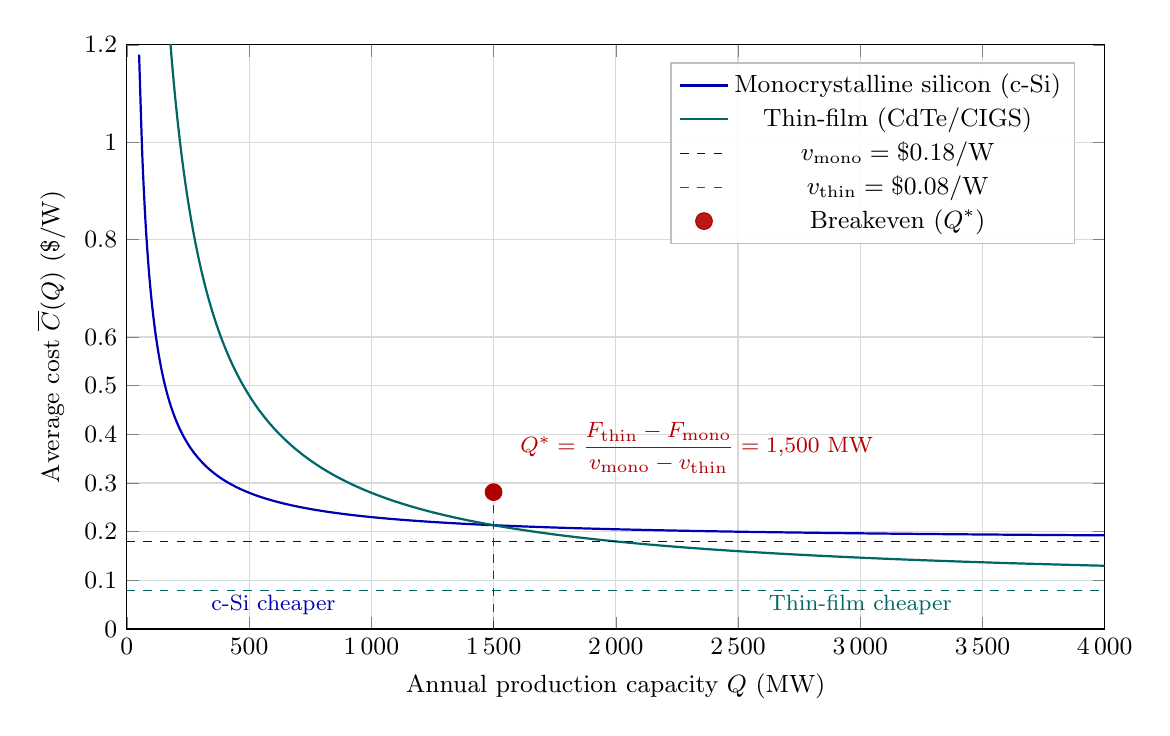
\begin{tikzpicture}
\begin{axis}[
    width=14cm,
    height=9cm,
    xlabel={Annual production capacity $Q$ (MW)},
    ylabel={Average cost $\overline{C}(Q)$ (\$/W)},
    xmin=0, xmax=4000,
    ymin=0, ymax=1.2,
    domain=50:4000,
    samples=300,
    grid=both,
    grid style={line width=0.2pt, draw=gray!20},
    major grid style={line width=0.4pt, draw=gray!30},
    legend style={
        at={(0.97,0.97)},
        anchor=north east,
        font=\small,
        draw=gray!50,
        fill=white,
        fill opacity=0.9,
        text opacity=1,
    },
    tick label style={font=\small},
    label style={font=\small},
    % Axis formatting
    scaled x ticks=false,
    x tick label style={/pgf/number format/1000 sep={\,}},
    y tick label style={/pgf/number format/fixed, /pgf/number format/precision=2},
    xtick={0,500,1000,1500,2000,2500,3000,3500,4000},
    ytick={0,0.10,0.20,0.30,0.40,0.50,0.60,0.80,1.00,1.20},
    clip=true,
]
 
% ---------------------------------------------------------------
%  Model: C_bar(Q) = F / Q + v
%
%  Parameters (illustrative; adjust to match your calibration):
%    c-Si:      F_mono = 50  ($M/yr),  v_mono = 0.18 ($/W)
%    Thin-film: F_thin = 200 ($M/yr),  v_thin = 0.08 ($/W)
%
%  Breakeven:  Q* = (F_thin - F_mono) / (v_mono - v_thin)
%                 = 150 / 0.10 = 1500 MW
% ---------------------------------------------------------------
 
% --- c-Si curve ---
\addplot[
    blue!70!black,
    thick,
    smooth,
] {50/x + 0.18};
\addlegendentry{Monocrystalline silicon (c-Si)}
 
% --- Thin-film curve ---
\addplot[
    teal!80!black,
    thick,
    smooth,
] {200/x + 0.08};
\addlegendentry{Thin-film (CdTe/CIGS)}
 
% --- Asymptotes (variable-cost floors) ---
\addplot[
    blue!70!black,
    dashed,
    thin,
    domain=0:4000,
] {0.18};
\addlegendentry{$v_{\mathrm{mono}} = \$0.18$/W}
 
\addplot[
    teal!80!black,
    dashed,
    thin,
    domain=0:4000,
] {0.08};
\addlegendentry{$v_{\mathrm{thin}} = \$0.08$/W}
 
% --- Breakeven point ---
\addplot[
    only marks,
    mark=*,
    mark size=3pt,
    red!70!black,
] coordinates {(1500, 0.2813)};
\addlegendentry{Breakeven ($Q^{*}$)}
 
% --- Vertical dashed line at breakeven ---
\draw[red!70!black, dashed, thin]
    (axis cs:1500, 0) -- (axis cs:1500, 0.2813);
 
% --- Annotation ---
\node[
    anchor=south west,
    font=\footnotesize,
    red!70!black,
    align=left,
] at (axis cs:1570, 0.30) {%
    $Q^{*} = \dfrac{F_{\mathrm{thin}} - F_{\mathrm{mono}}}{v_{\mathrm{mono}} - v_{\mathrm{thin}}} = 1{,}500$ MW%
};
 
% --- Region labels ---
\node[
    font=\footnotesize,
    blue!70!black,
    align=center,
] at (axis cs:600, 0.05) {c-Si cheaper};
 
\node[
    font=\footnotesize,
    teal!80!black,
    align=center,
] at (axis cs:3000, 0.05) {Thin-film cheaper};
 
\end{axis}
 
\end{tikzpicture}
\end{document}